\section{Specifications}
\label{sec:Specifications}

\newcounter{rulei}[subsection]
\newcommand{\rcnii}{\stepcounter{rulei}\arabic{section}.\arabic{subsection}.\arabic{rulei}}
\renewcommand{\labelenumi}{\rcnii}

\subsection{Markers}
\label{sub:markers}
The arena, tokens, pedestals, and robots involved in the game are labelled with \textit{libkoki} markers.
Each marker pattern encodes a number.
Each marker number is associated with a particular feature within the arena, and also has an associated size.
The marker numbers and sizes are as follows:

\begin{center}
  \begin{tabular}{lcc}
    \toprule
    \textbf{Item} & \textbf{Marker Numbers} & \textbf{Marker Size (mm)} \\
    \midrule
    Arena boundary & 0 -- 27 & 250 \\
    Robots & 28 -- 31 & 100 \\
    Pedestals & 32 -- 40 & 100 \\
    Tokens & 41 -- 64 & 250 \\
    \bottomrule
  \end{tabular}
\end{center}

Two sets of marker codes will be used: one for development purpose, and one for the competition itself.
The competition set is only to be used inside the Student Robotics arena at the Student Robotics competition.
This is so that people carrying markers past the arena do not confuse robots.
The competition codes are 100 above the development codes.
When run in competition mode (specifiable through the robot's GUI), the software provided by Student Robotics will subtract 100 from the detected marker codes, as well as ignore the development codes.

The markers can be printed on a black-and-white printer.
Marker designs can be downloaded from the documentation section of the Student Robotics website.

Unless specified otherwise, all markers described in this document are oriented vertically such that the principle corner of the marker (which is indicated by a dark grey dot in the black marker border) is on the higher edge.

\subsection{Robot Badges}
\label{sec:robot-badges}

\begin{figure}
  \centering
  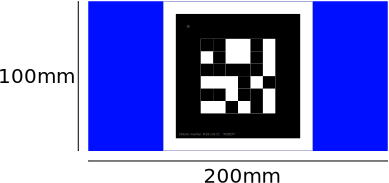
\includegraphics{./images/robot-marker.pdf}
  \caption{An example robot badge.
 The blue areas shown are the human-compatible areas.}
  \label{fig:example-badge}
\end{figure}

\begin{enumerate}
\item A ``robot badge'' is a removable identifier that will be attached to a robot throughout a match.
      It features the robot's assigned marker for the match, as well as human-compatible areas to allow spectators to easily associate a robot with its starting location.
      An example of one of these badges is shown in figure~\ref{fig:example-badge}.
      The markings in the human-compatible areas are intentionally not specified.

\item A robot must feature four of the badge mounts shown in figure~\ref{fig:badge-mounting}.
      These mounts must permit a flat $200 \times 100mm$ panel to be attached to them.
      The three areas of each mount must feature the illustrated areas of hook-type Velcro to allow this panel to be fitted.

\item The four badge mounts must be on the exterior of the robot, parallel with the vertical plane, and should be perpendicular to each other about the vertical axis\footnote{Teams can apply for a team-specific rule alteration to the required number of badges.
      Clear justification must be provided by the team with such a request.}
      The orientation of the badge mounts is unimportant, but teams are encouraged to position them horizontally as shown in figure~\ref{fig:example-badge}.

  \begin{figure}
    \centering
    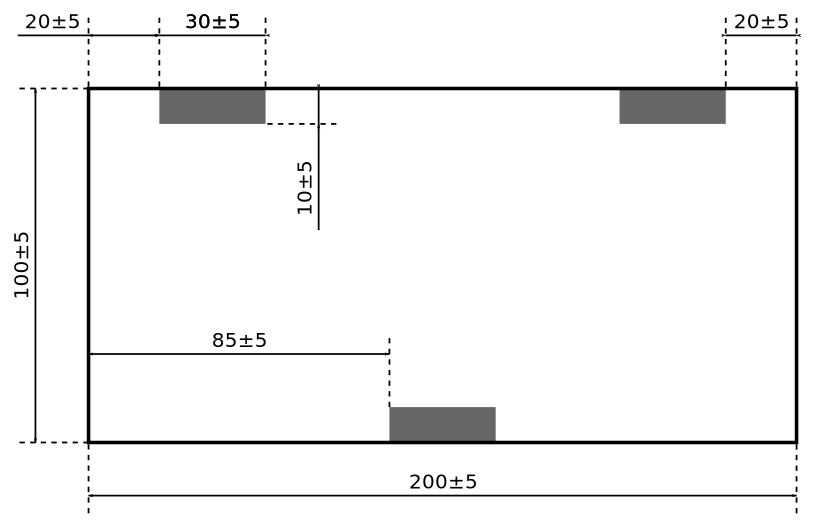
\includegraphics{./images/badge-mounting.pdf}
    \caption{The dimensions of the required robot badge mountings.
 The shaded areas are hook-type Velcro.
 All dimensions are in millimetres.}
    \label{fig:badge-mounting}
  \end{figure}
\end{enumerate}

\subsection{Arena}
\label{sub:arena}
\begin{enumerate}
\item The match arena floor, overall, is an $8m \times 8m$ square, as shown in figure~\ref{fig:arena-dim}.
      The tolerance of these two dimensions is $\pm0.25m$.

\begin{figure}
  \centering
  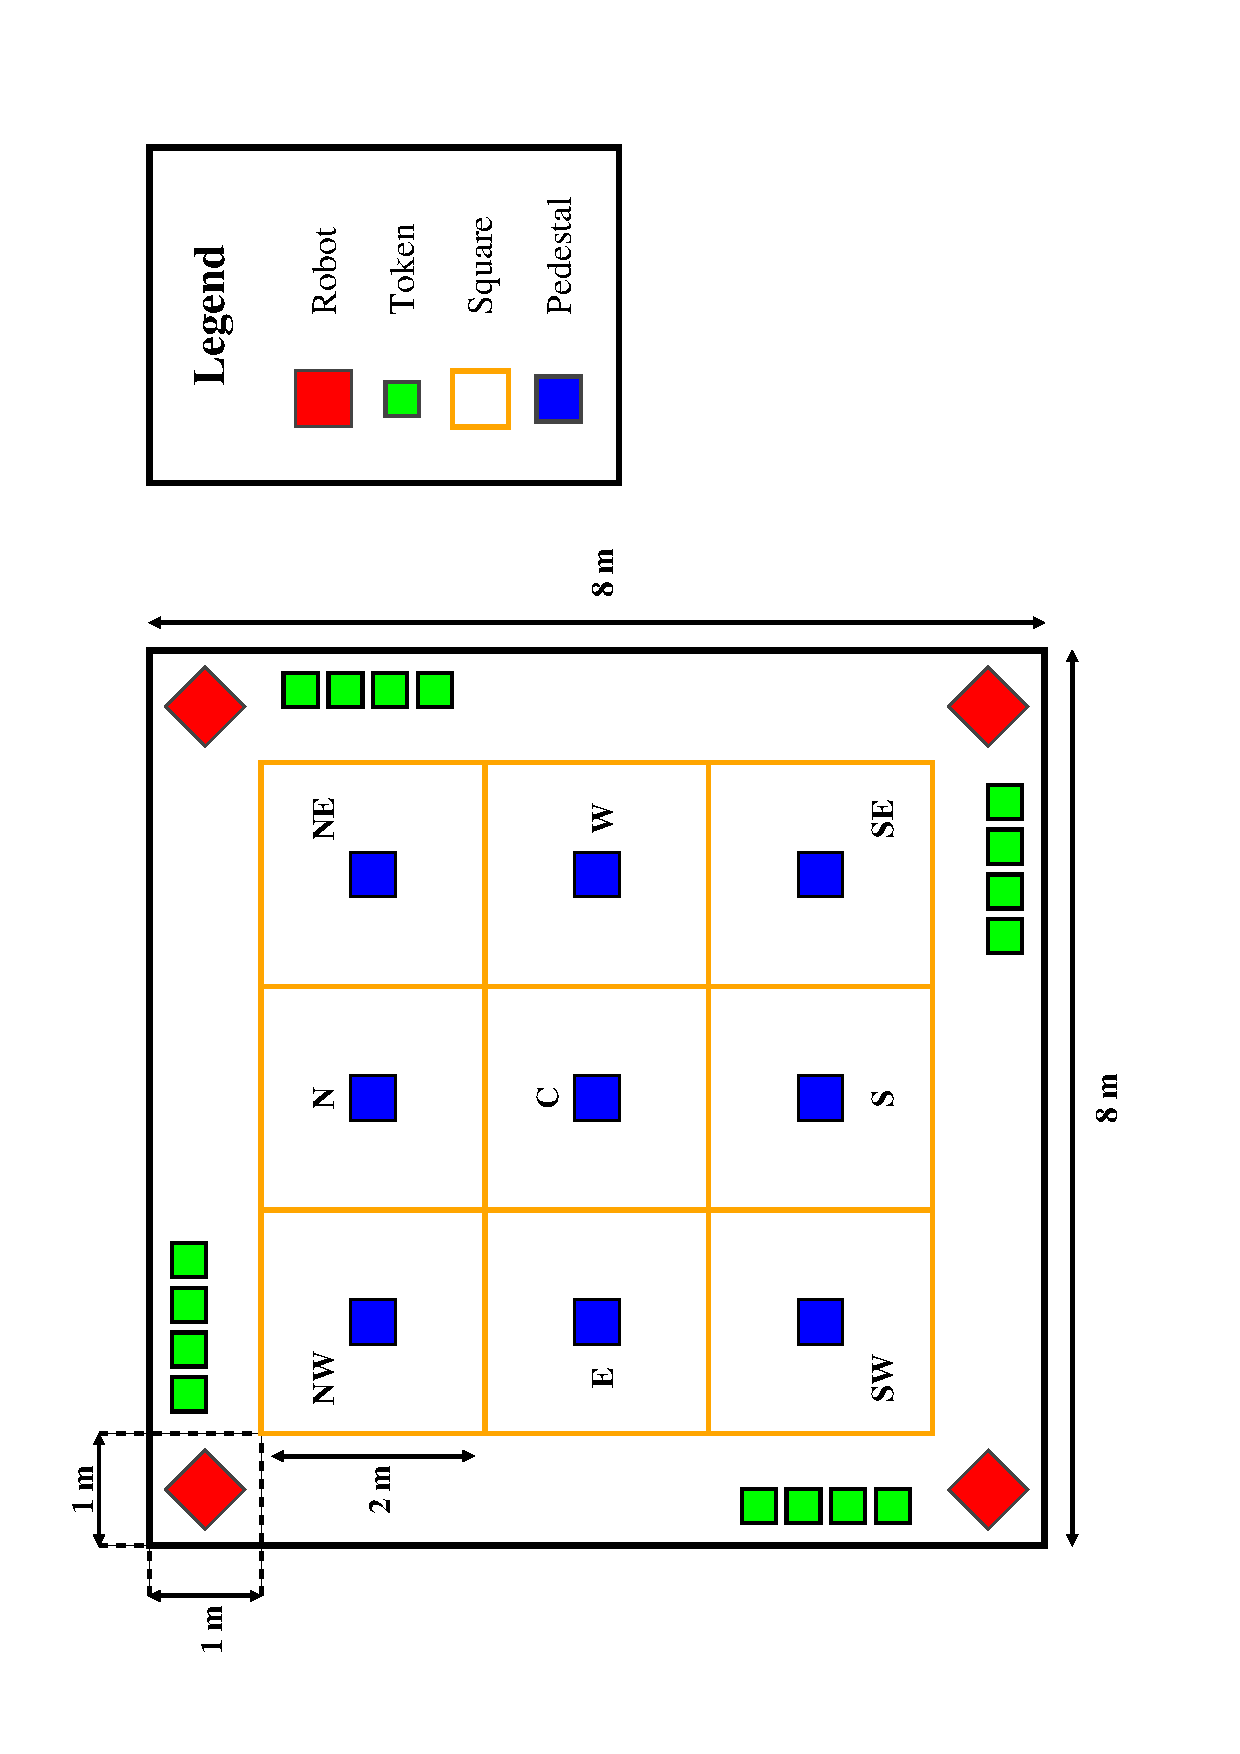
\includegraphics[width=0.8\textwidth, angle=270]{./images/arena.pdf}
  \caption{\label{fig:arena-dim}A bird's-eye view of the arena.}
\end{figure}

\item The floor of the arena is carpeted.
      The carpet tiles used in the arena are from B\&Q, with EAN 5014957151543.

\item The arena walls are $600\pm30mm$ high, the interior surfaces of which are white plastic-coated hardboard.

\item The arena features nine \textit{squares}.
      These areas are delineated by lines marked on the arena floor.
      The naming of these squares is shown in figure~\ref{fig:arena-zones}.

  \begin{figure}
    \centering
    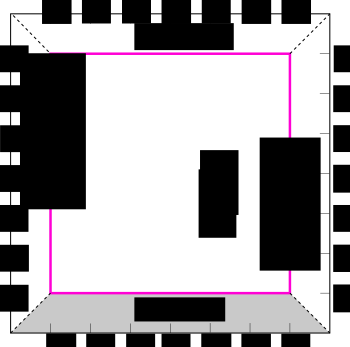
\includegraphics{./images/arena-markers.pdf}
    \caption{The positions and numbering of the markers positioned on the arena wall.}
    \label{fig:arena-zones}
  \end{figure}

\item Each wall of the arena features seven $250mm$ libkoki markers.
      Figure~\ref{fig:arena-wall} shows the positioning of these markers, whilst figure~\ref{fig:arena-zones} shows the numbering of these markers.

  \begin{figure}
    \centering
    
\includegraphics[width=\textwidth]{./images/sidewall.pdf}
    \caption{Seven $250mm$ wide markers are spaced evenly along each $8m$ arena wall.
             The markers are placed $50mm$ above the floor.}
    \label{fig:arena-wall}
  \end{figure}

\end{enumerate}

\subsection{Tokens}
\label{sub:Tokens}
\begin{enumerate}
\item Tokens are cubic corrugated cardboard boxes with side $305 \pm 15 mm$.
      \emph{Each team's kit contains two of these.}

\item Each token is associated with its own libkoki marker number.
      Each token is labelled with six identical $250mm$ libkoki markers -- one on each face.
\end{enumerate}

\subsection{Pedestals}
\label{sub:pedestals}
\begin{enumerate}
\item Pedestals are cubic structures of dimensions $320 \times 320 \times 320mm \pm 15mm$.
      The top of a pedestal is surrounded by a $20mm$ high rim to prevent tokens falling off.

\item Each pedestal features a $250mm$ marker in the centre of each vertical side.

\end{enumerate}

\clearpage
